{\small
  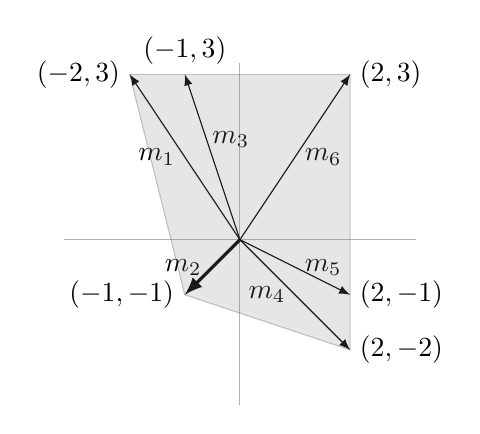
\begin{tikzpicture}[node distance=2cm,scale=0.7]
    \tikzstyle{lines}=[draw=black!30,rounded corners]
    \tikzstyle{vectors}=[-latex, rounded corners]
    \tikzstyle{rvectors}=[-latex,very thick, rounded corners]
    \draw[lines] (-3.2,0)--(3.2,0);
    \draw[lines] (0, 3.2)--(0,-3);
    \draw[vectors] (0, 0) --node[left]{$m_1$} (-2, 3) node[left]{$(-2,3)$};
    \draw[vectors] (0, 0) --node[left]{$m_4$} (2, -2)node[right]{$(2,-2)$};
    \draw[vectors] (0, 0) --node[right]{$m_6$} (2, 3)node[right]{$(2,3)$};
    \draw[rvectors] (0, 0) --node[left]{$m_2$} (-1, -1)node[left]{$(-1,-1)$};
    \draw[vectors] (0, 0) --node[above]{$~~~~m_3$} (-1, 3)node[above]{$(-1,3)$};
    \draw[vectors] (0, 0) --node[right]{$m_5$} (2, -1)node[right]{$(2,-1)$};

    \draw[fill=black!50,opacity=0.2] (-2,3) -- (-1,3) -- (2,3) --(2, -1) --(2,-2)
    -- (-1, -1) -- (-2, 3);
    
    
  \end{tikzpicture}
}
